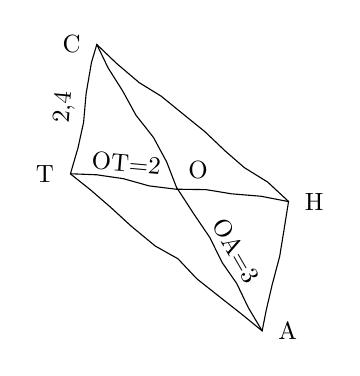
\begin{tikzpicture}[rotate=-60,every node/.style={scale=0.9},scale=0.7]

\coordinate (C) at (0,0);
\coordinate (H) at (4.21,1.59);
\coordinate (A) at (6,0);
\coordinate (T) at (1.79,-1.59);
\coordinate (O) at (3,0); %le centre du parallélogramme

\draw[decorate,decoration={random steps,amplitude=1pt,segment length=10pt}] (C) node [left=3pt]{C}--(H) node [right=3pt]{H} --(A) node [right=3pt] {A}--(T) node [left=3pt] {T}--cycle;
\draw [decorate,decoration={random steps,amplitude=1pt,segment length=10pt}] (C)--(A) (H)--(T);
\node at (O)[above right]{O}; 
\node at (4.5,0)[above,rotate=-60]{OA=3};
\path (C)--(T) node[midway,above,rotate=85]{2,4};
\path (T)--(O) node[midway,above,rotate=-5]{OT=2};

\end{tikzpicture}
